\chapter{Primo esercizio}

\section{Modello di Dominio}

\begin{center}
  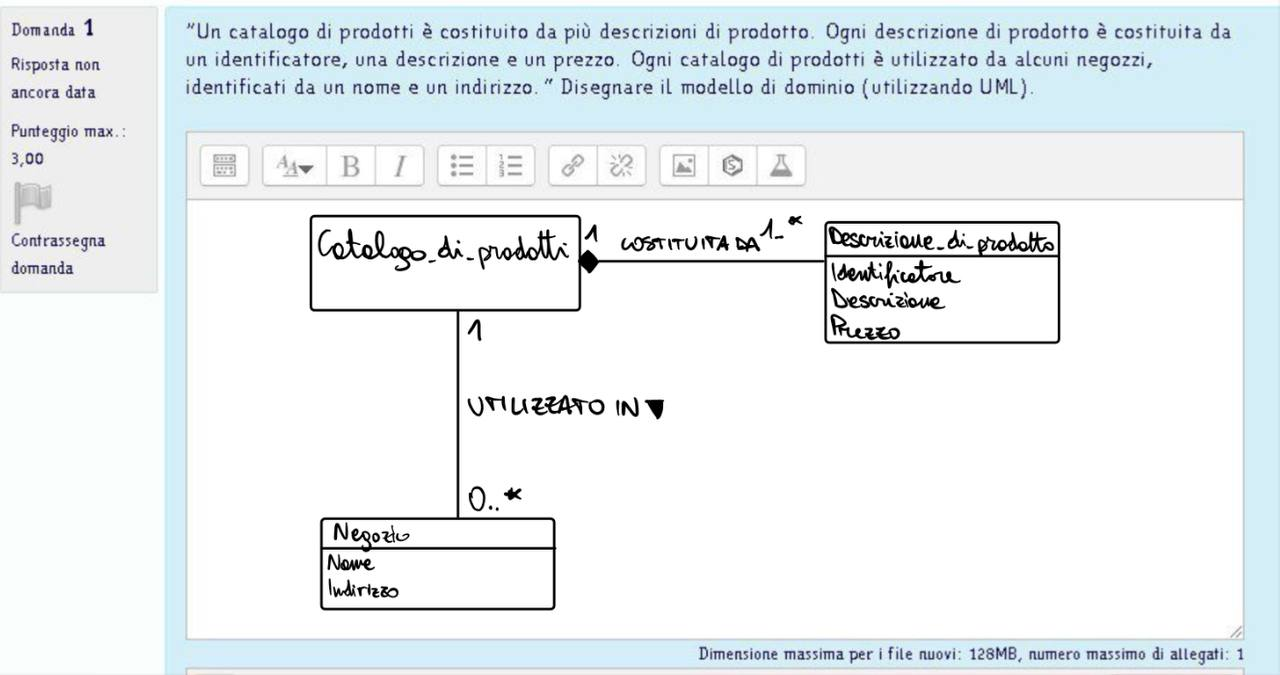
\includegraphics[scale=0.3]{ModelloDiDominio/ModelloDiDominio.jpg}
\end{center}

\section{SSD}

\qs{}{
  Si consideri il seguente scenario di base di Elabora Vendita:

  \begin{enumerate}
    \item il Cliente arriva alla cassa POS con gli articoli e/o i servizi da acquistare;
    \item il Cassiere inizia una nuova vendita;
    \item il Cassiere inserisce il codice identificativo di un articolo;
    \item il Sistema registra la riga di vendita per l'articolo e mostra una descrizione dell'articolo, il suo prezzo e il totale parziale;
    \item il Cassiere ripete i passi 3-4 fino a che non indica che ha terminato;
    \item il Sistema mostra il totale;
    \item il Cassiere riferisce il totale al Cliente e richiede il pagamento;
    \item il Cliente paga (in contanti) e il sistema gestisce il pagamento;
    \item il sistema registra la vendita completata;
    \item il Sistema genera la ricevuta;
    \item il Cliente va via con la ricevuta e gli articoli acquistati.
  \end{enumerate}
}

\nt{Fare attenzione al rumore bianco: non tutti i passi forniscono informazioni utili per la realizzazione del SSD.}

\begin{center}
  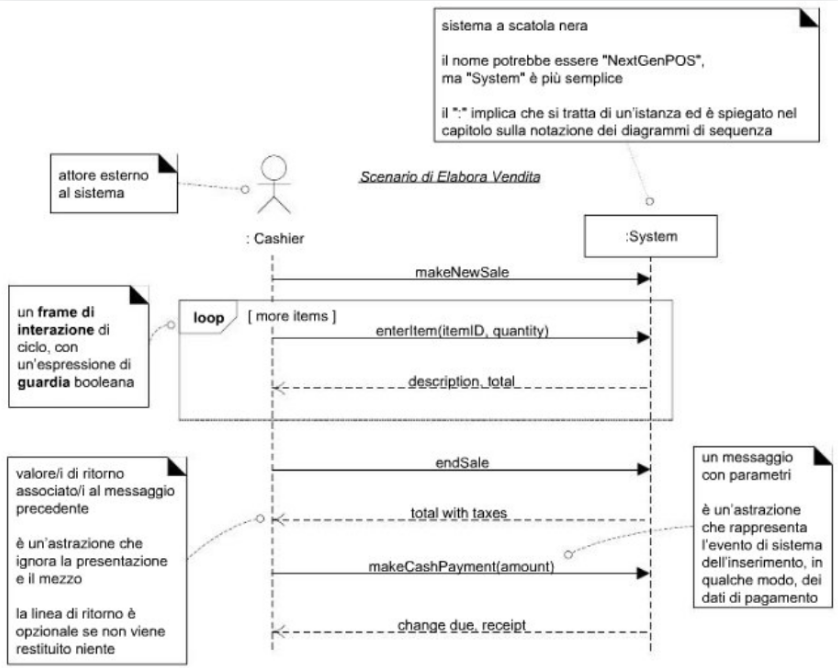
\includegraphics[scale=0.7]{SSD/SSD.png}
\end{center}

\section{Contratti}

\qs{}{Definire in modo preciso la pre-condizione e la post-condizione di un'operazione di Sistema. Fare un esempio di operazione con le sue pre-condizioni e le sue post-condizioni.}

\dfn{Pre-condizioni}{Ipotesi significative sullo stato del sistema o degli oggetti nel Modello di
Dominio prima dell’esecuzione dell'operazione. Si tratta di ipotesi non banali, che
dovrebbero essere comunicate al lettore.}

\dfn{post-condizioni}{È la sezione più importante. Descrive i cambiamenti di stato degli
oggetti nel Modello di Dominio dopo il completamento dell’operazione.
}

\ex{enterItem}{

  \paragraph{Pre-condizioni:}
  \begin{itemize}
    \item [$\Rightarrow$] è in corso una vendita $s$.
  \end{itemize}

  \paragraph{Post-condizioni:}
  \begin{itemize}
    \item [$\Rightarrow$] è stata creata un'istanza $sli$ di SalesLineItem;
    \item [$\Rightarrow$] $sli$ è stata associata con la Sale corrente $s$;
    \item [$\Rightarrow$] $sli$ è stata associata con una ProductDescription, in base alla corrispondenza con ItemID;
    \item [$\Rightarrow$] $sli.quantity$ è diventatat $quantity$.
  \end{itemize}

}

\section{DSD}

\begin{center}
  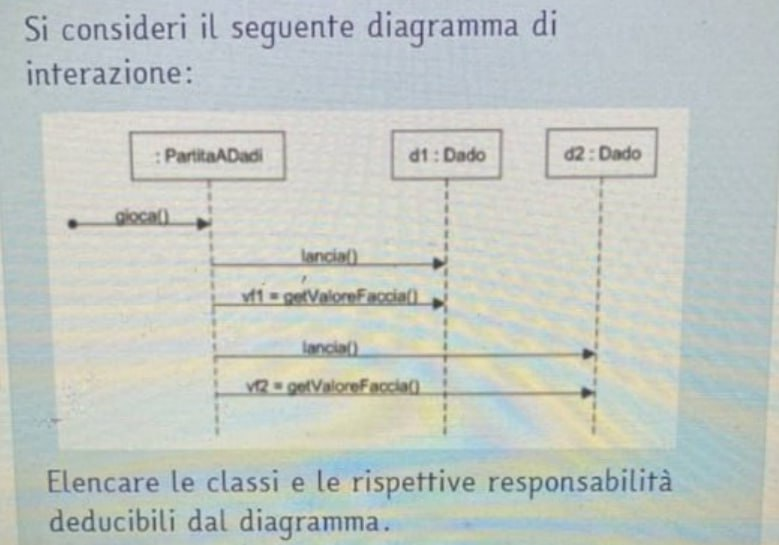
\includegraphics[scale=0.7]{DSD/DSD.jpg}
\end{center}
\paragraph{Le classi coinvolte sono:}

\begin{itemize}
  \item [$\Rightarrow$] \texttt{PartitaADadi};
  \item [$\Rightarrow$] \texttt{Dado}.
\end{itemize}

\texttt{PartitaADadi} è il GRASP controller perchè si occupa di chiamare i metodi (delegandoli) sulle altre classi per coordinarle. \texttt{PartitaADadi} ha la responsabilità di conoscere le classi \texttt{Dado}. Ogni Classe \texttt{Dado} ha la responsabilità di conoscere il valore uscito sulla propria faccia dopo il lancio (il \texttt{Dado} è l'\textit{esperto delle informazioni} rispetto a quel valore).

\begin{center}
  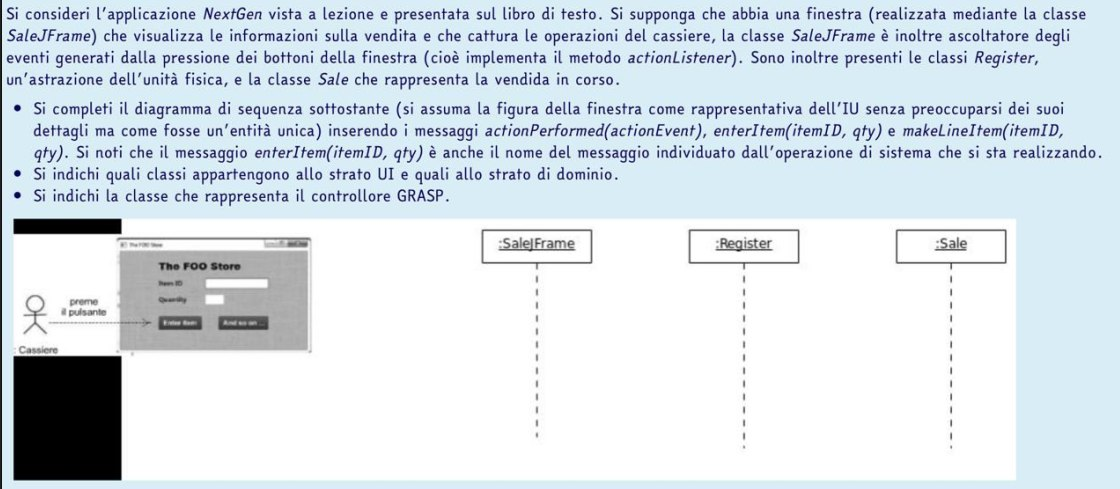
\includegraphics[scale=0.5]{DSD/DSD2.jpg}
\end{center}

\nt{
  \begin{itemize}
    \item \textbf{Strato UI:} \texttt{SaleJFrame};
    \item \textbf{Strato di Dominio:} \texttt{Register} e \texttt{Sale}.
  \end{itemize}
  Il GRASP controller è \texttt{Register}.
}

\begin{center}
  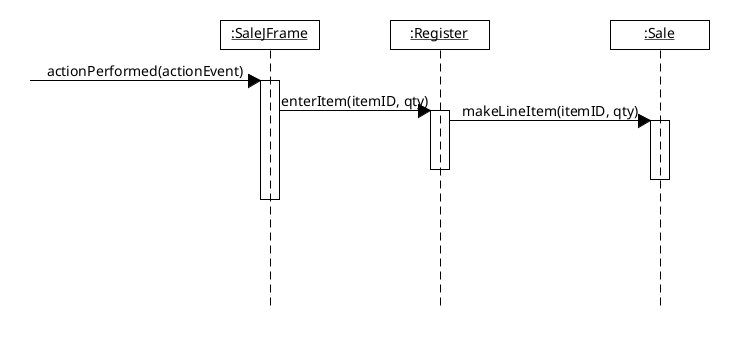
\includegraphics[scale=0.4]{DSD/DSD2.png}
\end{center}

\section{DSD}


\begin{center}
  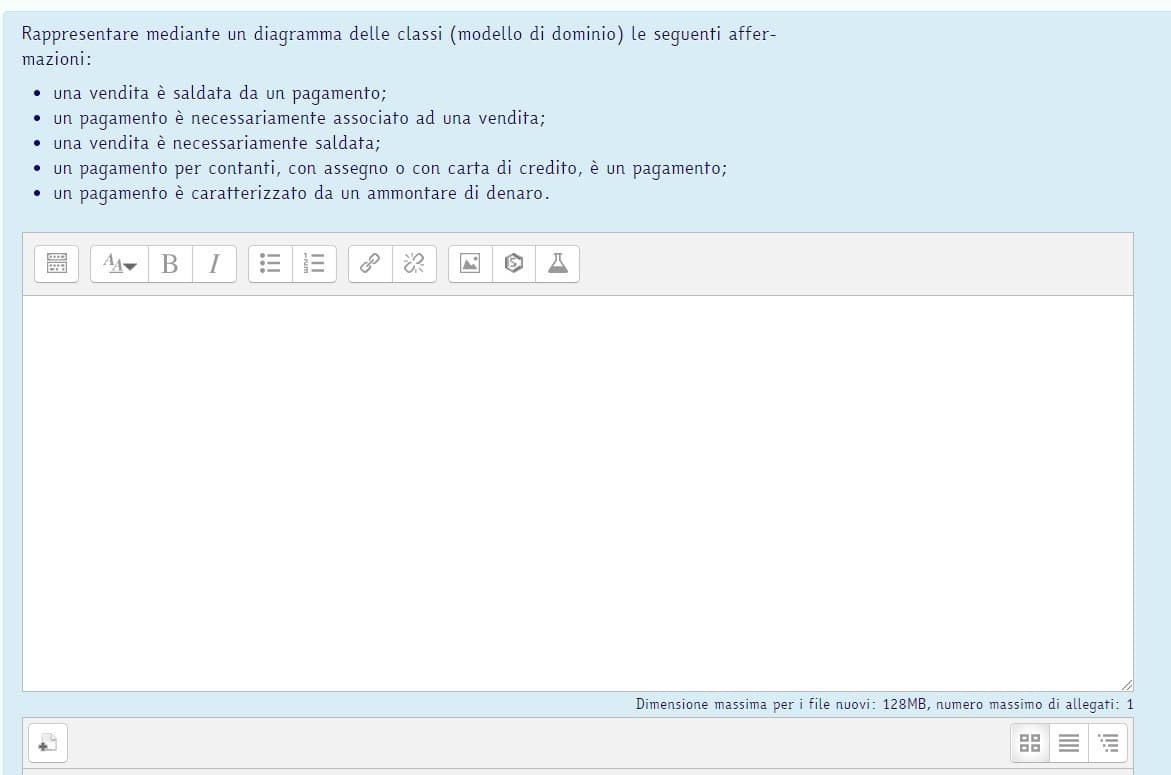
\includegraphics[scale=0.4]{DCD/DCD.jpg}
\end{center}

\nt{Prestare attenzione alle cardinalità. Poiché una vendita è obbligatoriamente saldata l'unica cardinabilità disponibile è 1. Per lo stesso motivo, dato che un pagamento salda una sola vendita anche l}

\begin{center}
  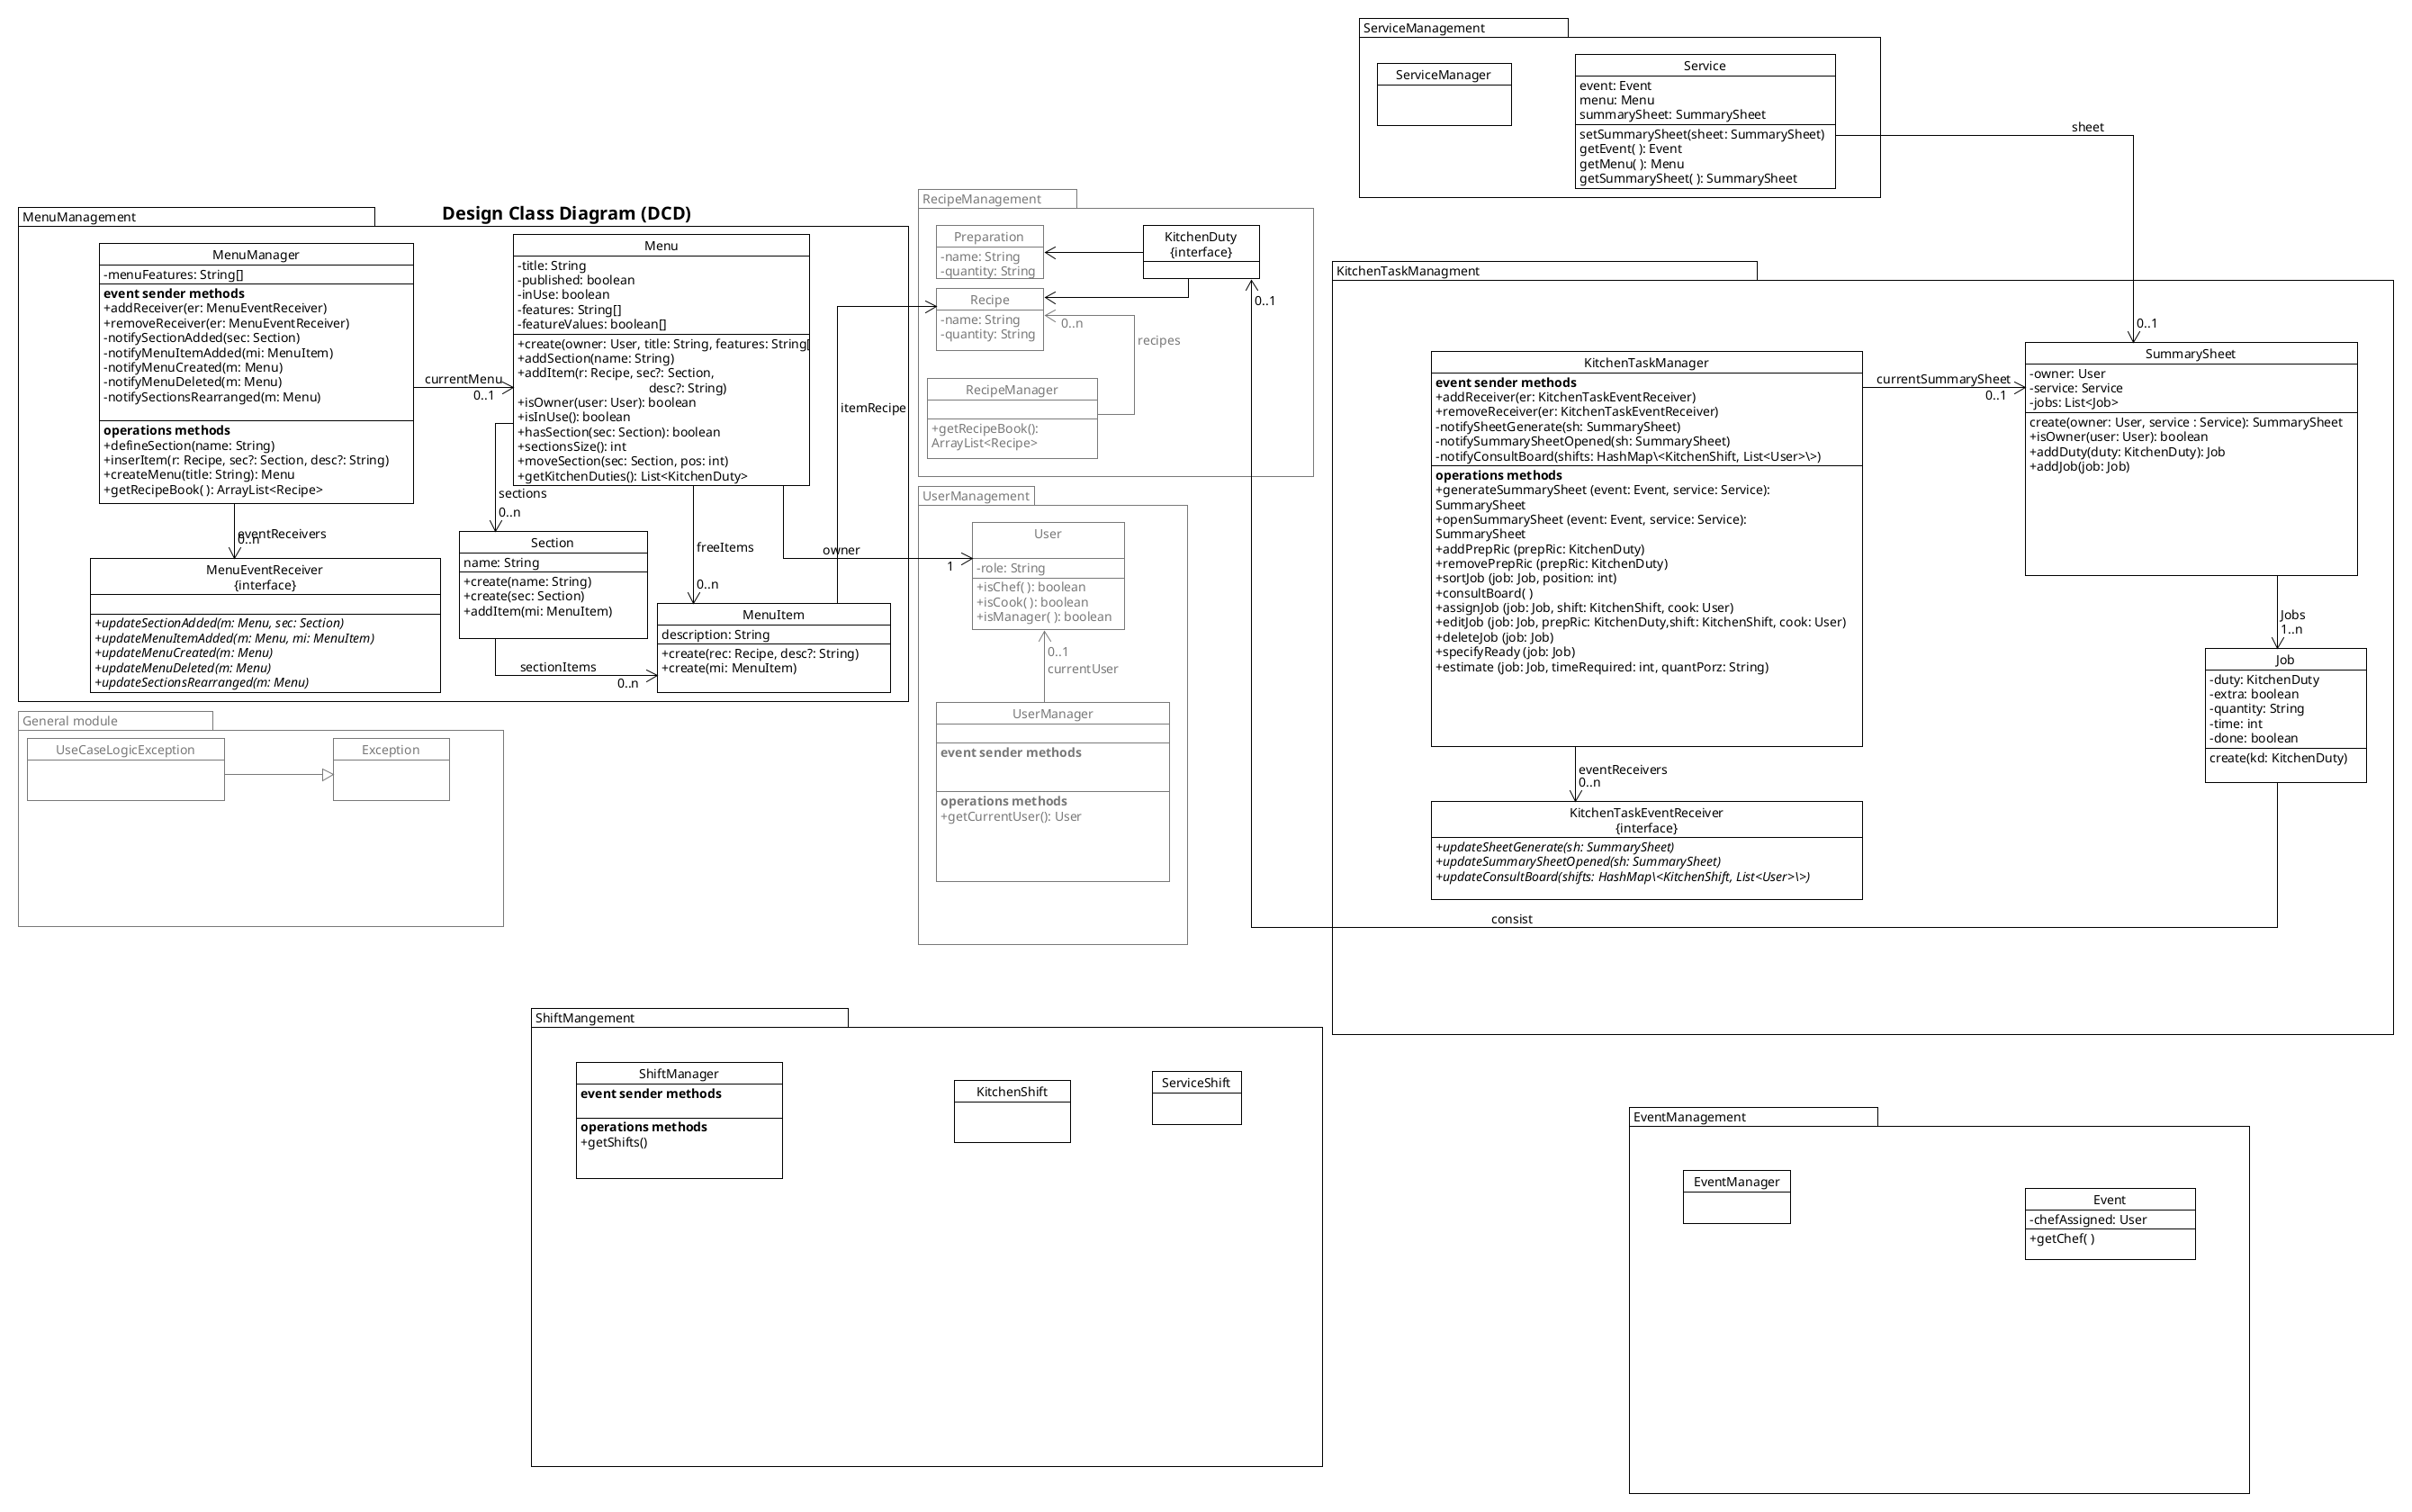
\includegraphics[scale=0.5]{DCD/DCD.png}
\end{center}
